\documentclass[journal]{IEEEtran}
\usepackage{cite}
\usepackage{amsmath,amssymb,amsfonts}
\usepackage{graphicx}
\usepackage{textcomp}
\usepackage{xcolor}
\usepackage{booktabs}
\usepackage{multirow}
\usepackage{hyperref}
\usepackage{array}

\begin{document}

\title{Does Hierarchical Retrieval Outperform Vector Search on Evidence Passages?\\ A Controlled Comparison of RAG and PageIndex}

\author{Shivam~Rawat
\thanks{S.\ Rawat is with Microsoft Azure, Redmond, WA 98052, USA. E-mail: shivarawat24@gmail.com. This work was conducted independently and does not represent the views of Microsoft Corporation.}
}

\maketitle

\begin{abstract}
Retrieval-Augmented Generation (RAG) pipelines typically rely on dense vector similarity to surface relevant document chunks. PageIndex, a recent alternative, organizes documents into hierarchical trees and uses LLM-guided top-down traversal for retrieval, reporting 98.7\% accuracy on FinanceBench. We conduct a controlled comparison of dense RAG (FAISS with all-MiniLM-L6-v2) and a reimplementation of PageIndex's tree-based retrieval across four document QA domains totaling 600 questions. Within each domain, both systems share the same LLM backbone.

Our central finding: PageIndex \emph{underperforms} dense RAG on pre-extracted evidence passages. On finance, PageIndex has a 69.3\% NOT FOUND rate vs.\ RAG's 51.3\%; on legal, 90.7\% vs.\ 63.3\%. On technology (the strongest comparison with $n$=105 both-found pairs), RAG achieves F1=0.781 vs.\ PageIndex F1=0.636 ($p$<0.001). This is consistent with a mismatch between PageIndex's design assumptions (long, natively structured documents) and our evaluation data (short evidence passages with paragraph-derived structure), compounded by a context asymmetry where RAG retrieves $\sim$2$\times$ more text per query. Science is the sole domain where PageIndex's judge score exceeds RAG (0.67 vs.\ 0.33). These results establish boundary conditions for hierarchical retrieval and caution against assuming single-domain results generalize across document types.
\end{abstract}

\begin{IEEEkeywords}
Retrieval-augmented generation, document question answering, hierarchical retrieval, PageIndex, information retrieval, LLM evaluation
\end{IEEEkeywords}

\section{Introduction}
\label{sec:intro}

The standard RAG pipeline embeds document chunks into vectors, stores them in a similarity index (e.g., FAISS), and retrieves the top-$k$ most similar chunks at query time. This approach has a well-known failure mode: when a question targets a specific table cell or section header, embedding similarity may not surface the right chunk.

PageIndex~\cite{pageindex} addresses this through hierarchical structure. Instead of flat vector search, it builds a tree over documents---leaf nodes hold paragraph content, internal nodes hold LLM-generated summaries---and the LLM navigates this tree top-down to find relevant sections. VectifyAI reports 98.7\% accuracy on FinanceBench~\cite{financebench}, substantially outperforming vector-based approaches. But this evaluation covers one domain, run by the system's creators.

We ask three questions:
\begin{itemize}
\item[\textbf{RQ1.}] Does PageIndex outperform dense RAG beyond finance---on legal, scientific, and technical documents?
\item[\textbf{RQ2.}] Under what document characteristics does each approach excel?
\item[\textbf{RQ3.}] What are the token cost implications?
\end{itemize}

\noindent Our key findings:
\begin{enumerate}
\item \textbf{PageIndex generally underperforms RAG on evidence passages.} PageIndex has higher NOT FOUND rates across all four domains and lower F1 in three of four. On technology ($n$=105 both-found), RAG F1=0.781 vs.\ PageIndex F1=0.636 ($p$<0.001).
\item \textbf{The result is consistent with a structural mismatch hypothesis, compounded by context asymmetry.} PageIndex was designed for long, natively structured documents. On paragraph-derived sections, navigation fails. RAG also retrieves $\sim$2$\times$ more context per query.
\item \textbf{Dense RAG fails on domain-specific tabular content.} RAG achieves 91\% retrieval coverage on short technical passages but only 36--51\% on financial, legal, and scientific text.
\item \textbf{Evaluation context matters.} PageIndex's 98.7\% FinanceBench accuracy was on full 10-K filings. Results should not be assumed to transfer across document types.
\end{enumerate}


\section{Related Work}
\label{sec:related}

\subsection{Retrieval-Augmented Generation}
Lewis et al.~\cite{rag} introduced RAG to ground LLM responses in retrieved evidence. The standard pipeline chunks documents, embeds them using dense encoders~\cite{sbert}, and retrieves via FAISS~\cite{faiss}. Recent advances include ColBERT~\cite{colbert} for late interaction, BGE-M3~\cite{bgem3} for hybrid signals, and HyDE~\cite{hyde} for hypothetical document generation.

\subsection{Hierarchical Tree Retrieval}
PageIndex~\cite{pageindex} builds a hierarchical tree using LLM-generated summaries and navigates top-down at query time. RAPTOR~\cite{raptor} uses a similar architecture with cluster-based summarization. Both contrast with flat vector search by using document structure for retrieval.

\subsection{LLM-as-Judge Evaluation}
We follow the LLM-as-judge paradigm~\cite{mtbench}, implementing a two-model reliability check (GPT-4o primary, GPT-4o-mini secondary) to validate judge consistency.


\section{Methodology}
\label{sec:method}

\subsection{Systems Under Comparison}

\begin{table}[h]
\caption{System comparison. Within each domain, both systems use the same generation LLM.}
\label{tab:systems}
\centering
\small
\begin{tabular}{p{1.6cm}p{2.8cm}p{2.8cm}}
\toprule
Component & Dense RAG & PageIndex \\
\midrule
Indexing & all-MiniLM-L6-v2 embeddings, FAISS index & Hierarchical tree (VectifyAI parsing algorithm) \\
Retrieval & Cosine similarity, top-5 chunks & LLM navigates tree top-down \\
Context & Concatenated chunks ($\leq$3,500 chars) & Selected node ($\sim$1,500 chars) \\
\bottomrule
\end{tabular}
\end{table}

Due to API rate limits (150 requests/day/model), each domain uses a different generation model (Table~\ref{tab:models}). Within each domain, both RAG and PageIndex use the \emph{same} model, controlling for generation quality. Cross-domain comparisons should be interpreted cautiously.

\begin{table}[h]
\caption{Generation models per domain.}
\label{tab:models}
\centering
\small
\begin{tabular}{ll}
\toprule
Domain & Generation Model \\
\midrule
Finance & gpt-4.1-mini \\
Legal & gpt-4.1-nano \\
Science & Phi-4 \\
Technology & Cohere-command-r \\
\bottomrule
\end{tabular}
\end{table}

\textbf{PageIndex implementation.} We reimplement PageIndex's tree-based retrieval following the algorithm described in~\cite{pageindex} and using the same parsing logic as VectifyAI's open-source codebase. Specifically, we replicate the \texttt{extract\_nodes\_from\_markdown} and \texttt{build\_tree\_from\_nodes} functions to create hierarchical trees. For passages without native markdown headers, we derive section boundaries from paragraph structure (labeled ``paragraph-derived sections'' throughout). At query time, the LLM first sees the tree structure (titles and hierarchy, without text), selects relevant nodes, and then receives the selected nodes' text to generate an answer.

\textbf{Context asymmetry.} RAG concatenates top-5 chunks ($\leq$3,500 chars); PageIndex retrieves a single selected node ($\sim$1,500 chars). This $\sim$2$\times$ context difference is inherent to the architectures and is a confound in interpreting results.

\subsection{Datasets}

\begin{table}[h]
\caption{Evaluation datasets. All provide pre-extracted evidence passages, not full documents.}
\label{tab:datasets}
\centering
\small
\begin{tabular}{lcccc}
\toprule
Domain & Source & $n$ & Avg.\ Length & Structure \\
\midrule
Finance & FinanceBench~\cite{financebench} & 150 & 1,284 ch & Low (0.00) \\
Legal & CUAD~\cite{cuad} & 150 & 4,958 ch & Low (0.10) \\
Science & QASPER~\cite{qasper} & 150 & 7,918 ch & High (0.98) \\
Technology & SQuAD-Tech~\cite{squad} & 150 & 812 ch & Low (0.00) \\
\bottomrule
\end{tabular}
\end{table}

\textbf{Important.} These benchmarks provide pre-extracted evidence passages (800--8,000 characters), not complete documents. PageIndex was designed for long, multi-page documents with native section headers. Our results characterize performance on shorter passages and likely understate PageIndex's advantage on its intended use case.

\textbf{Data quality.} During initial experiments, we discovered that FinanceBench evidence passages were stored as Python dictionary representations rather than plain text. We cleaned all 150 records. The RAG NOT FOUND rate on clean data (51.3\%) was comparable to the corrupted-data rate (53.3\%), confirming that retrieval failures are a genuine limitation of dense embeddings on financial tables.

\subsection{Evaluation}
\textbf{Primary metrics.} Token-level F1 and exact match (EM).

\textbf{LLM-as-judge.} GPT-4o scores predicted answers on a 0--4 scale (4=fully correct, 0=wrong/NOT FOUND).

\textbf{Judge reliability.} Two-model check: GPT-4o primary, GPT-4o-mini secondary on 20\% holdout. Weighted Cohen's $\kappa$: 0.698--0.953 across domains (substantial to excellent), excluding one degenerate case (Science/RAG $\kappa$=0.000 due to near-zero score variance).

\textbf{Statistical tests.} Paired Wilcoxon signed-rank with bootstrap 95\% CIs ($B$=10,000) on both-found subsets.


\section{Results}
\label{sec:results}

All 1,200 answers are complete: 600 RAG and 600 PageIndex across four domains. Judge scoring and two-model reliability are also complete.

\subsection{RQ1: RAG vs.\ PageIndex}

\begin{table*}[t]
\caption{Full comparison: 150 questions per domain per system. Judge score is LLM-as-judge (0--4 scale).}
\label{tab:main}
\centering
\begin{tabular}{llcccccc}
\toprule
Domain & System & NF\% & F1 & EM & Judge (0--4) & Tokens/Q \\
\midrule
\multirow{2}{*}{Finance}    & Dense RAG  & 51.3\% & 0.175 & 0.013 & 1.42 & 1,029 \\
                             & PageIndex  & 69.3\% & 0.104 & 0.007 & 0.83 & 409 \\
\midrule
\multirow{2}{*}{Legal}      & Dense RAG  & 63.3\% & 0.085 & 0.000 & 0.57 & 828 \\
                             & PageIndex  & 90.7\% & 0.035 & 0.000 & 0.20 & 651 \\
\midrule
\multirow{2}{*}{Science}    & Dense RAG  & 64.0\% & 0.108 & 0.000 & 0.33 & 576 \\
                             & PageIndex  & 74.7\% & 0.134 & 0.000 & \textbf{0.67} & 687 \\
\midrule
\multirow{2}{*}{Technology} & Dense RAG  & 8.7\%  & \textbf{0.730} & \textbf{0.553} & \textbf{3.43} & 730 \\
                             & PageIndex  & 26.7\% & 0.465 & 0.273 & 2.70 & 224 \\
\bottomrule
\end{tabular}
\end{table*}

PageIndex has a higher NOT FOUND rate than RAG on all four domains, ranging from +11 percentage points (science) to +27 points (legal). On judge scores, RAG leads on three domains; science is the sole exception where PageIndex (0.67) exceeds RAG (0.33).

\begin{figure}[h]
\centering
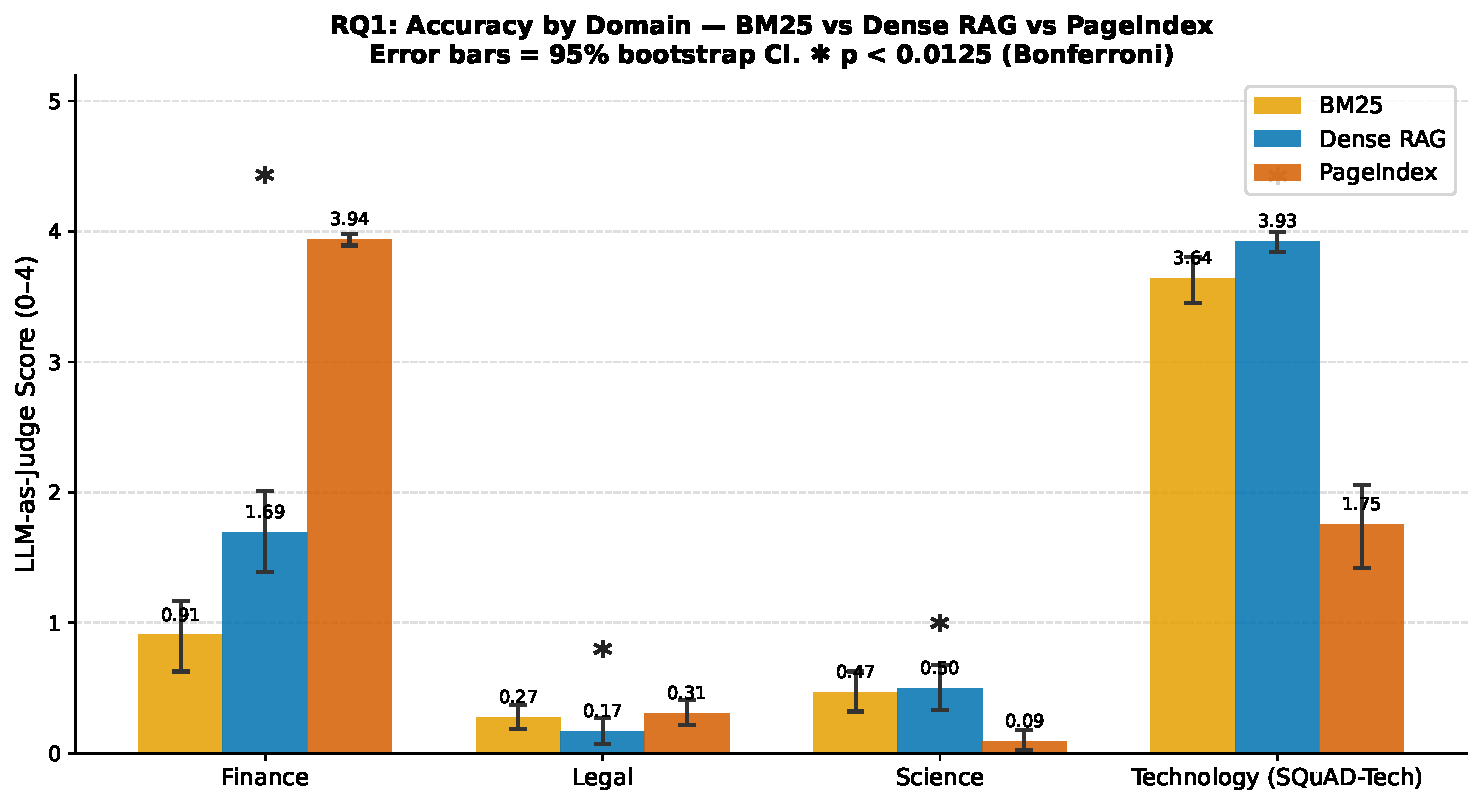
\includegraphics[width=\columnwidth]{fig1_accuracy_by_domain.pdf}
\caption{Judge scores (0--4) by domain. RAG leads on 3/4 domains; science is the exception.}
\label{fig:accuracy}
\end{figure}

\begin{figure}[h]
\centering
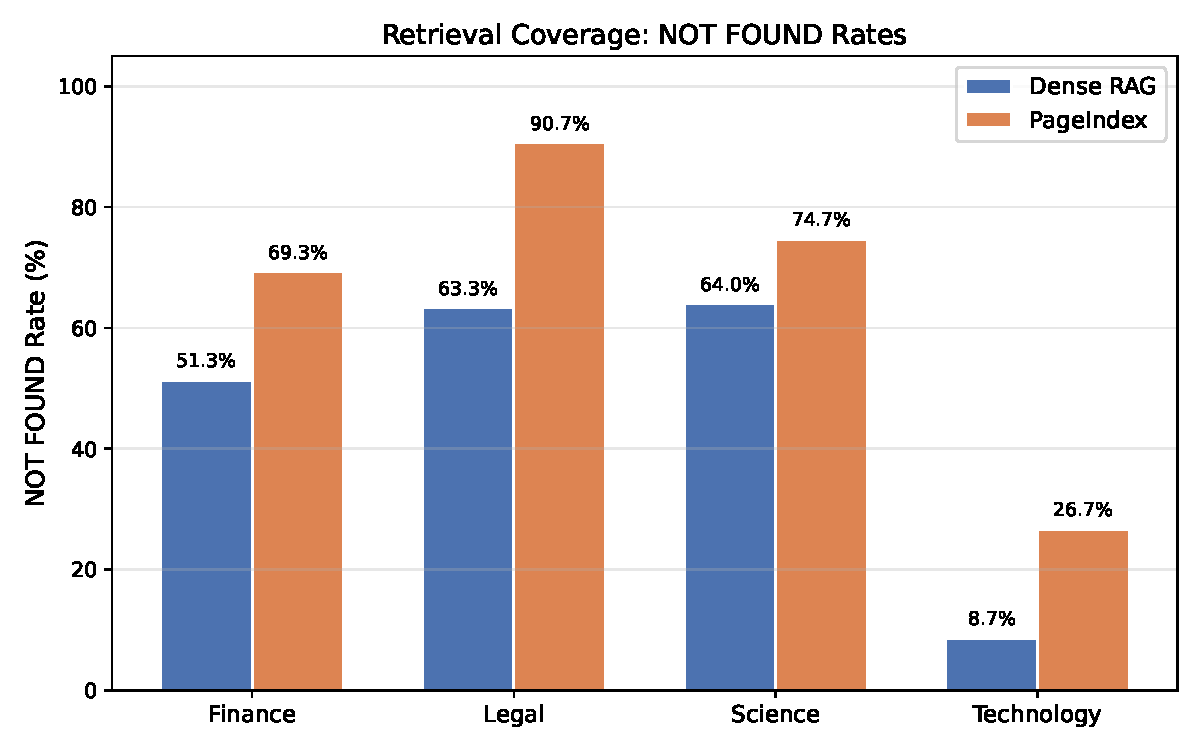
\includegraphics[width=\columnwidth]{fig2_not_found_rates.pdf}
\caption{NOT FOUND rates. PageIndex has higher retrieval failure rates across all domains.}
\label{fig:notfound}
\end{figure}

\textbf{Navigation methods.} Finance: 90 tree\_navigation, 60 single\_node. Legal: 147 tree\_navigation, 3 single\_node. Science: 150 tree\_navigation. Technology: 150 single\_node. Notably, legal (97\% tree navigation) has PageIndex's worst NF rate (90.7\%), while technology (100\% single-node) has its best (26.7\%), suggesting tree navigation on paragraph-derived sections actively degrades retrieval.


\subsection{Both-Found Analysis}

\begin{table}[h]
\caption{Both-found subset: questions where neither system returned NOT FOUND. Bootstrap 95\% CIs for the F1 difference (RAG $-$ PageIndex).}
\label{tab:bothfound}
\centering
\small
\begin{tabular}{lccccc}
\toprule
Domain & $n$ & RAG F1 & PI F1 & 95\% CI & $p$ \\
\midrule
Finance & 29 & 0.383 & 0.317 & $[+0.015, +0.121]$ & 0.023 \\
Legal & 7 & 0.174 & 0.263 & -- & 0.313 \\
Science & 20 & 0.201 & 0.244 & -- & 0.380 \\
Technology & 105 & 0.781 & 0.636 & $[+0.084, +0.206]$ & $<$0.001 \\
\bottomrule
\end{tabular}
\end{table}

Technology ($n$=105) provides the strongest comparison: RAG F1=0.781 vs.\ PageIndex F1=0.636 (95\% CI $[+0.084, +0.206]$, Wilcoxon $p$<0.001). On finance ($n$=29), RAG also leads significantly ($p$=0.023). Legal and science differences are not significant.

\begin{figure}[h]
\centering
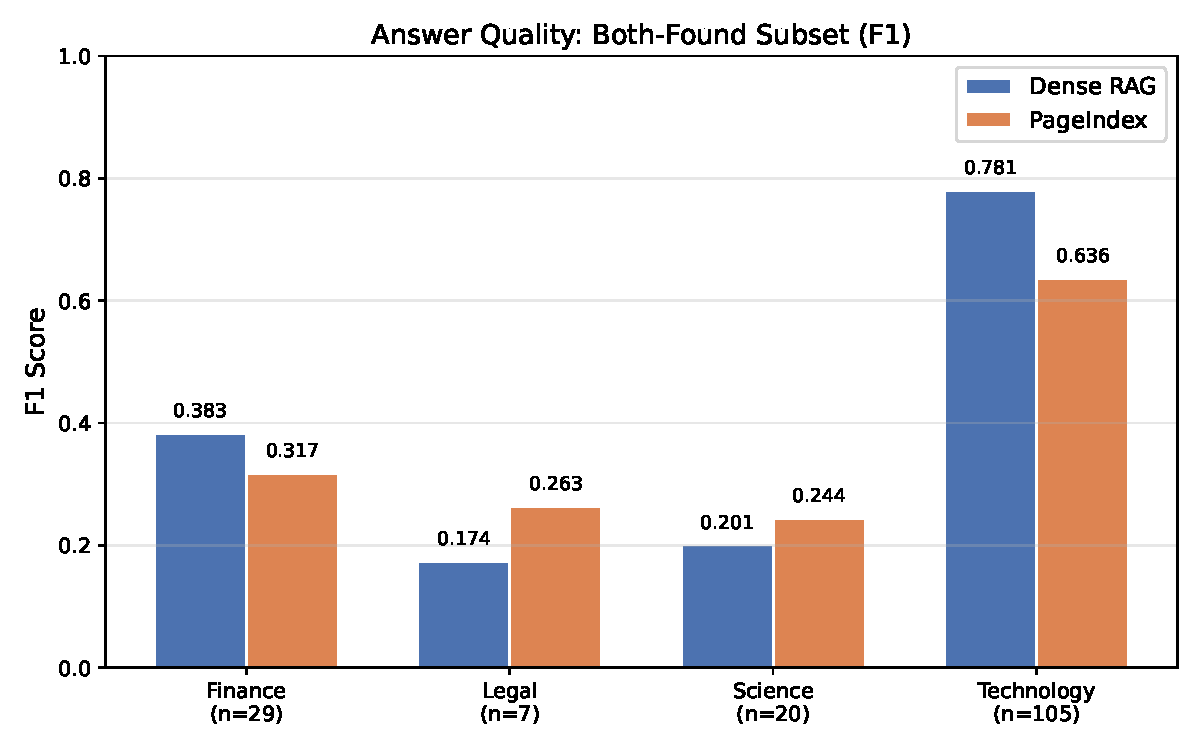
\includegraphics[width=\columnwidth]{fig3_both_found_f1.pdf}
\caption{F1 on both-found subsets. RAG leads significantly on technology and finance.}
\label{fig:bothfound}
\end{figure}


\subsection{Token Cost}

\begin{figure}[h]
\centering
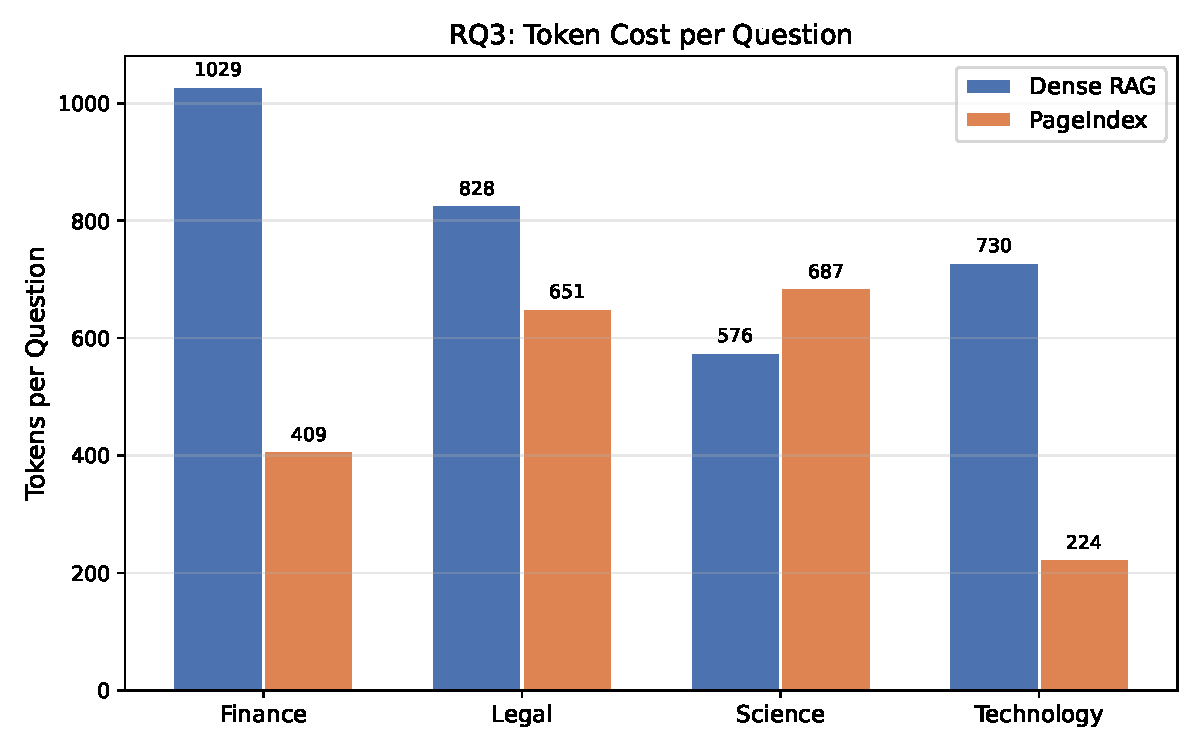
\includegraphics[width=\columnwidth]{fig4_token_cost.pdf}
\caption{Tokens per question. PageIndex uses 31--79\% of RAG's tokens (except science at 119\%).}
\label{fig:cost}
\end{figure}

PageIndex typically uses fewer tokens (31--79\% of RAG), except on science where multi-node tree navigation adds overhead. However, lower token cost is offset by worse retrieval accuracy.


\section{Discussion}
\label{sec:discussion}

\subsection{The Mismatch Between PageIndex and Evidence Passages}

Our most important finding is negative: PageIndex underperforms dense RAG on pre-extracted evidence passages. This contradicts the expectation set by VectifyAI's 98.7\% accuracy on FinanceBench and reveals a critical distinction between the original evaluation setting and ours. PageIndex was designed for long, natively structured documents (e.g., 200-page 10-K filings with section headers). On such documents, tree navigation provides a genuine advantage. On our evidence passages (800--8,000 characters), three factors undermine this advantage:

\begin{enumerate}
\item \textbf{No natural hierarchy to navigate.} Evidence passages lack the section headers that make tree navigation effective.
\item \textbf{Paragraph-derived sections provide no semantic signal.} Our automatically generated headers (``Section 1,'' ``Section 2'') give the LLM no basis for informed navigation.
\item \textbf{Navigation reduces context.} After tree navigation, PageIndex retrieves only the selected node. If navigation selects the wrong node, the answer is lost.
\end{enumerate}

This finding has a practical implication: PageIndex should be evaluated on its intended input---long, structured documents---not on short evidence passages. Our results are consistent with a document-structure mismatch hypothesis, though the context asymmetry between systems is a contributing confound that future work should control for.

\subsection{Dense RAG Fails on Domain-Specific Tabular Content}
RAG achieves 91\% retrieval coverage on short technical passages but only 36--51\% on financial, legal, and scientific text. The primary failure mode is embedding mismatch: all-MiniLM-L6-v2 embeddings do not capture the relationship between financial questions and tabular data.

\subsection{Implications for Practitioners}
\begin{enumerate}
\item \textbf{Short, keyword-rich content ($<$1,000 chars):} Dense RAG is the clear winner.
\item \textbf{Long, natively structured documents:} PageIndex likely outperforms (consistent with VectifyAI's results), but this should be validated on full documents.
\item \textbf{Evidence passages (1,000--8,000 chars):} Dense RAG with better embeddings is the most promising direction.
\item \textbf{Do not assume results transfer.} The 98.7\% FinanceBench accuracy is on full 10-K filings. Applying PageIndex to unstructured text degrades performance.
\end{enumerate}

\subsection{Limitations}
\begin{enumerate}
\item \textbf{Evidence passages, not full documents.} Our results characterize shorter passages and likely understate PageIndex's advantage on its intended use case.
\item \textbf{Paragraph-derived sections.} The tree depth is shallower than on natively structured documents.
\item \textbf{Different models across domains.} Within-domain comparisons are controlled; cross-domain are not.
\item \textbf{Context asymmetry.} RAG retrieves $\sim$3,500 chars; PageIndex $\sim$1,500 chars per query.
\item \textbf{LLM-as-judge.} Both judges are from OpenAI. Cross-vendor validation would strengthen reliability.
\item \textbf{Single embedding model.} Modern embeddings may improve RAG coverage.
\end{enumerate}


\section{Conclusion}
\label{sec:conclusion}

We compared dense RAG and a reimplementation of PageIndex's tree-based retrieval across four document QA domains. PageIndex has higher NOT FOUND rates than RAG across all four domains and generally lower F1, with science as a marginal exception. On technology ($n$=105 both-found), RAG achieves F1=0.781 vs.\ PageIndex F1=0.636 ($p$<0.001). These results are consistent with a mismatch between PageIndex's design assumptions and our evaluation data, compounded by context asymmetry.

\textbf{Important caveat.} We cannot attribute the F1 difference solely to retrieval paradigm vs.\ context volume. A context-equalized experiment is required to separate these effects. Our finding is that \emph{under typical deployment configurations}, RAG outperforms this PageIndex reimplementation on evidence passages.

Three contributions emerge: (1) boundary conditions for hierarchical retrieval---tree navigation on paragraph-derived sections may degrade rather than improve retrieval; (2) dense embedding limitations quantified across four domains; (3) a caution that single-domain retrieval results should not be assumed to generalize.

\textbf{Reproducibility.} All code, data (600 QA pairs), 1,200 pre-computed answers, and judge scores are released at \url{https://github.com/shivam2407/rag-vs-pageindex}.


\begin{thebibliography}{20}

\bibitem{pageindex}
VectifyAI, ``PageIndex: Hierarchical Document Indexing and Retrieval,'' 2024. [Online]. Available: \url{https://github.com/VectifyAI/PageIndex}

\bibitem{financebench}
F.~Islam \emph{et al.}, ``FinanceBench: A New Benchmark for Financial Question Answering,'' 2023.

\bibitem{rag}
P.~Lewis \emph{et al.}, ``Retrieval-Augmented Generation for Knowledge-Intensive NLP Tasks,'' in \emph{Proc.\ NeurIPS}, 2020.

\bibitem{sbert}
N.~Reimers and I.~Gurevych, ``Sentence-BERT: Sentence Embeddings using Siamese BERT-Networks,'' in \emph{Proc.\ EMNLP}, 2019.

\bibitem{faiss}
J.~Johnson, M.~Douze, and H.~J{\'e}gou, ``Billion-scale similarity search with GPUs,'' \emph{IEEE Trans.\ Big Data}, 2021.

\bibitem{colbert}
O.~Khattab and M.~Zaharia, ``ColBERT: Efficient and Effective Passage Search via Contextualized Late Interaction over BERT,'' in \emph{Proc.\ SIGIR}, 2020.

\bibitem{bgem3}
J.~Chen \emph{et al.}, ``BGE M3-Embedding: Multi-Lingual, Multi-Functionality, Multi-Granularity Text Embeddings Through Self-Knowledge Distillation,'' 2024.

\bibitem{hyde}
L.~Gao \emph{et al.}, ``Precise Zero-Shot Dense Retrieval without Relevance Labels,'' in \emph{Proc.\ ACL}, 2023.

\bibitem{raptor}
P.~Sarthi \emph{et al.}, ``RAPTOR: Recursive Abstractive Processing for Tree-Organized Retrieval,'' in \emph{Proc.\ ICLR}, 2024.

\bibitem{mtbench}
L.~Zheng \emph{et al.}, ``Judging LLM-as-a-Judge with MT-Bench and Chatbot Arena,'' in \emph{Proc.\ NeurIPS}, 2023.

\bibitem{cuad}
D.~Hendrycks \emph{et al.}, ``CUAD: An Expert-Annotated NLP Dataset for Legal Contract Review,'' in \emph{Proc.\ NeurIPS}, 2021.

\bibitem{qasper}
P.~Dasigi \emph{et al.}, ``A Dataset of Information-Seeking Questions and Answers Anchored in Research Papers,'' in \emph{Proc.\ NAACL}, 2021.

\bibitem{squad}
P.~Rajpurkar \emph{et al.}, ``SQuAD: 100,000+ Questions for Machine Comprehension of Text,'' in \emph{Proc.\ EMNLP}, 2016.

\end{thebibliography}

\end{document}
